\documentclass[10pt,twocolumn,letterpaper]{article}

% My own stuff
\usepackage{booktabs}
% \usepackage{caption}
% \captionsetup[table]{skip=8pt}   % Only affects tables
\usepackage{stfloats}  % Add this to the preamble
\usepackage{float}
\usepackage{xeCJK}  % Supports Simplified & Traditional Chinese
\setCJKmainfont{IPAMincho} 

\usepackage{cvpr}
\usepackage{times}
\usepackage{epsfig}
\usepackage{graphicx}
\usepackage{amsmath}
\usepackage{amssymb}

% Include other packages here, before hyperref.

% If you comment hyperref and then uncomment it, you should delete
% egpaper.aux before re-running latex.  (Or just hit 'q' on the first latex
% run, let it finish, and you should be clear).
\usepackage[breaklinks=true,bookmarks=false]{hyperref}

\cvprfinalcopy % *** Uncomment this line for the final submission

\def\cvprPaperID{****} % *** Enter the CVPR Paper ID here
\def\httilde{\mbox{\tt\raisebox{-.5ex}{\symbol{126}}}}

% Pages are numbered in submission mode, and unnumbered in camera-ready
%\ifcvprfinal\pagestyle{empty}\fi
\setcounter{page}{1}
\begin{document}

%%%%%%%%% TITLE
\title{ECDOデータ駆動型プライマーパート1/2: 発熱性核-マントル離脱ジャンニベコフ振動(ECDO)“地球反転”理論の現状理解}

\author{ジュンホ\\
ウェブサイト: \href{https://sovrynn.github.io}{sovrynn.github.io}\\
ECDOリサーチリポジトリ: \href{https://github.com/sovrynn/ecdo}{github.com/sovrynn/ecdo}\\
{\tt\small junhobtc@proton.me}
}

\maketitle
%\thispagestyle{empty}

%%%%%%%%% ABSTRACT
\begin{abstract}
2024年5月、"The Ethical Skeptic"という偽名のオンライン著者が、発熱性核-マントル離脱ジャンニベコフ振動(ECDO)という画期的な理論を共有しました \cite{0}。この理論は、地球が以前に回転軸の突然の重大な変動を経験し、その結果、回転慣性によって海が大陸を覆い尽くし、世界的な洪水を引き起こしたことを示唆しています。加えて、別の反転が差し迫っている可能性を示す説明的な地球物理学的プロセスとデータを提示しています。このような大洪水と世界滅亡の予測は新しくありませんが、ECDO理論は、科学的で現代的、学際的、そしてデータに基づくアプローチのため、特に説得力があります。

本論文は、6か月にわたるECDO理論に関する独立した研究の要約の第一部です \cite{2,20}。3つの重要な点を強調しています:

\begin{flushleft}
\begin{enumerate}
    \item 人類の最近の歴史において、ECDOのような「地球反転」が複数回発生したことが、洪水神話や広範な大陸洪水の地質学的証拠によって示されています。
    \item 過去の地球反転のおおよその方向と規模を特定することができます。
    \item 最近の地磁気および地球物理学データは、別の地球反転が差し迫っている可能性を示唆しており、気候変動が人間ではなく地球内部深くの変化によって引き起こされる可能性があります。
\end{enumerate}
\end{flushleft}

加えて、ECDO理論によって提案された「地球反転」の原因物理学を取り上げます。

この論文では、ハードデータに焦点を当てることで客観性を保ち、理論の惹きつけられるが投機的な部分を避け、人類がもっと調査する必要がある急務の課題であることを強調します。
\end{abstract}

%%%%%%%%% BODY TEXT
\section{はじめに}

大洪水の話は珍しくなく、実際、地球上の主要な文明の発祥地を含むすべての主要文化に見られます。267の洪水物語の集積をプロットする(図\ref{fig:1})と、実際に人が住む地球上のほとんどの地域に洪水の物語が存在することがわかります。

\begin{figure}[h]
\begin{center}
   \includegraphics[width=1\linewidth]{b.png}
\end{center}
   \caption{世界中の洪水物語の位置 \cite{3}.}
\label{fig:1}
\label{fig:onecol}
\end{figure}

これらの洪水物語を詳しく見ると、これらは通常の洪水ではなく、大陸を一掃する洪水を伴った破壊的な大異変であったことがわかります。

\subsection{ネイティブアメリカンの大異変物語}

ネイティブアメリカンの物語には、地球の大異変の最も生々しい証言のいくつかが含まれています。アリゾナ州北東部に住むネイティブアメリカンの部族ホピ族は、「ソトゥクナンは選ばれた人々のためにアリ族に地下世界を開かせた。彼らが無事に地下に入ると、ソトゥクナンは双子のポカングホヤとパロンガウホヤに、地軸の北端と南端に配置されていた彼らの持ち場を離れるよう命じた。 \textbf{双子が持ち場を離れた途端、地球は制御する者なしにバランスを崩し、不規則に回転し、そして二回転した。} 山は大きな波とともに海に沈み、海や湖は陸地を覆いました。そして、地球は冷たく命のない宇宙空間を回転して、堅い氷になりました」と言います\cite{4}。

これらの物語の多くは、洪水の大規模さを正確に述べており、どうやって海が最高の山頂を除いて全てを覆うまで上昇したかを語っています。ワシントン州に住むスココミッシュ族はこう語ります。「偉大なる霊は人々と動物たちの悪逆非道を怒り、良い動物、一人の良い男とその家族以外を地上から一掃することに決めた。偉大なる霊の指示で、その男は雲に向かって矢を射り、その矢にまた矢を射り、こうして雲から地面まで矢のロープを作った。良い動物と人々が登り始めた。悪い動物や蛇も登り始めたが、男はロープを断ち切った。 \textbf{その後、偉大なる霊は何日も雨を降らせ、タコマ(マウント・レーニア)の雪線まで洪水を起こした。} 悪人たちと悪い動物たちがすべて溺れた後、偉大なる霊は雨を止め、水がゆっくりと引き、良い人々と動物たちが降りて行った」と\cite{3}。参考までに、マウント・レーニアはワシントン州にある標高4392.5メートルの活火山です。

ワシントン州のマカ族の洪水物語は、特に「非常に暖かい」水の多段階洪水を述べており、これは通常の洪水ではないことを示しています。「海が高く上昇し、岬を切り離しました。次にそれは後退し、四日間の低潮の後、ニア湾を高く乾いた状態にしました。次にそれは再び上昇し、山頂以外を覆いました。\textbf{上昇する水は非常に暖かかった。} カヌーを持つ人々は持ち物を積み込み、北へ遠く運ばれました。カヌーが木に捕らえられて多くが亡くなりました。四日後、海は正常に戻り、人々は遠く北へ運ばれたことに気づきました。彼らの子孫は今もそこに住んでいます」と\cite{3}。

\subsection{中国の大異変物語}

太平洋の反対側では、現代の中国文明は大洪水から始まったと言われています。紀元前2000年頃に存在したと推定される夏王朝は、禹王によって作られ、彼が鯀・禹の大洪水を止めたとされています\cite{6}。彼の時代に、「... 10日間も太陽が沈まないという奇跡が起こり、森林が燃え上がり、多数の忌まわしい虫が出現した... 天に達するほどの巨大な波が中国の地に降り注いだ。 \textbf{"水は高い山々にまで達し、ふもとは全く見えなかった"}... "洪水の氾濫は破壊的だ"と皇帝は言った。 "その広大な範囲で山々を抱覆し、高い峰を越えて、洪水と共に天を脅かす。" 皇帝は、山々の間の谷に留まっている水を放出するためのすべての努力を命じた。多くの年にわたり、人口は大洪水の水から平野や谷を解放しようとして、チャネルを掘り、田畑を排水することに従事しました。相当な数の年の間、すべての努力は無駄でした。この緊急で巨大な作業を担当していた担当大臣の鯀は失敗のために死刑判決を受け... そして彼の息子禹だけが土地を排水することに成功しました。この業績は非常に高く評価され、禹は堯の後継者である舜の後、中国の皇帝となりました" \cite{5}。

中国だけでなく洪水があり、地球の回転が洪水中に変わったことを示唆するように、方位や太陽と月の動きを再測定する必要があったようです。: \textit{\textbf{"この皇帝は学者を中国の異なる地域やさらにはインドシナに送って、太陽の昇る方角と沈む方角、星の動きを観察することによって北・西・東・南の位置を確認させた。} また、彼は天文学者に季節の期間を調べ、新しい暦を作成するように命じた... "そこで堯[堯]は唐と豢に命じて、広大な天空に敬意を払って、太陽、月、星々の動きと姿を計算し、描くようにさせ、人々に季節を丁重に知らせるように命じた"} \cite{5}。

中国の歴史における大変動の記録は実際には夏王朝よりもはるか以前、三皇五帝の時代まで遡ります\cite{7}。三皇の一人であり中国史における創造の中心人物である女媧は、地球の回転が変わる大変動の中で洪水を止めました: \textit{"より力の強い2人の神の間で争いがあり、彼らはそれを戦いで解決することに決めました。水神共工が負けを悟ると、彼は頭を不周山に打ち付けました。 不周山は天を支えている柱で、その柱が崩れた結果、天が西北に傾き、地球が南東に移動しました。このため、終わりのない火災、広大な洪水、人を食らう獰猛な獣の出現などの大災害が引き起こされました。 女媧は巨大な亀の足を切り取り、それを倒れた柱の代用品として使い、状況を多少改善し、7色の石で割れた空を封じましたが、傾いた空を完全に直すことはできませんでした"} \cite{8}。

\subsection{ヨーロッパ、マヤ、中東、東南アジアの大変動故事}

多くの大災害物語の詳細をこの論文内で述べるには数が多すぎるため、そのような物語を持つ他の著名な文化のいくつかを簡単に紹介します。ギリシャ文学にはデウカリオン、オギュゲス、ダルダヌスの3つの洪水物語があります\cite{9,10}。前者の伝説では、\textit{"九日間の洪水の後、世界は破壊され、箱舟は標高2,457メートルのパルナソス山の頂上に止まった"}というものです\cite{11}。マヤ文学では、現在の太陽の前に4つの異なる太陽があったと信じており、4番目の太陽カルチウートリクエの時代は、紀元前3100年頃の世界を滅ぼす洪水と現在の5番目の太陽の誕生で終わったとされています\cite{12}。中東では、聖書の年代記に有名なノアの洪水が含まれていますし、バビロニアの叙事詩ギルガメシュには似たような話があります\cite{13}。東南アジアの文化もまた洪水物語が豊富です。たとえば、インドネシアのオト・ダヌム族は、\textit{"大洪水がかつて多くの人々を溺死させた。数人が船で逃れて、水上に残る唯一の山頂に到達し、そこで三ヶ月暮らした後、洪水が引いた"}と語っています\cite{3}。彼らの住むボルネオ島の最高地点は4,095メートルです。

\begin{figure*}[b]
\begin{center}
% \fbox{\rule{0pt}{2in} \rule{.9\linewidth}{0pt}}
\includegraphics[width=1\textwidth]{marine.jpg}
\end{center}
   \caption{海洋(海の)化石、塩水、塩田/鉱山のグローバルプロット\cite{15,16,86,87}。}
   \label{fig:2}
\end{figure*}

\subsection{統計的な大災害物語の分析}

明らかに、これらの物語は他の種類の壊滅的な地球物理的力を伴った洪水を描写しています。117の大災害物語(表\ref{tab: 1})の分析では、大規模な洪水と共に火事、地形の変化、地球の回転の変化が共に記録されることが多いことを示しています\cite{14}:

\begin{table}[ht]
\begin{center}
\renewcommand{\arraystretch}{1.2}  % Optional, to increase row spacing
\begin{tabular}{|l|c|c|}
\hline
\textbf{大災害の種類} & \textbf{数} & \textbf{発生率\%} \\
\hline\hline
洪水/大水害            & 84 & 71.79 \\
炎上/火災            & 39 & 33.33 \\
地形の変化           & 29 & 24.79 \\
星の混乱              & 15 & 12.82 \\
空の崩壊              & 15 & 12.82 \\
長期にわたる暗闇        & 14 & 11.97 \\
失われた土地と湖      & 12 & 10.26 \\
暴風                   & 10 & 8.55  \\
軸の/回転の変化      & 9  & 7.69  \\
沸騰する川/湖/海      & 8  & 6.84 \\
\hline
\end{tabular}
\end{center}
\caption{物語における壊滅的な影響の発生}
\label{tab: 1}
\end{table}

世界中の多くの独立した文化から出現する洪水物語の具体性と、他の大災害の出来事の一致する物語は、これらの洪水物語が実際に起こった災害の直接的な記録である可能性を示唆しています。

\section{海洋洪水の物理的証拠}

洪水物語を裏付けるのは、地球の大陸表面に広がる広範な海洋洪水のさまざまな物理的証拠です。その最も直接的な証拠の形式には、塩(塩水、塩田、塩鉱)や海洋(海の)化石が含まれ、地球の大陸地塊の広範な地域を覆っています。図\ref
いくつかの塩水を含む最も興味深い地域は、チベットのヒマラヤの高地と南米のアンデス山脈であり、どちらも平均高度4000メートルの地域で、前者は図\ref{fig:3}に描かれています。チベットの洪水の物語では、\textit{"\textbf{チベットはほぼ完全に水没したが}、神のギャが生き残った人々に憐れみを持ち、ベンガルを通じて水を引き、水が猿よりもほとんど上回らない人々を文明化させるために教師を送りました。" } \cite{3}と語られています。ペルーの神話では、山の上の洪水と共に山の造成が起こることが記述されています。\textit{"羊飼いは彼の6人の子供とすべての食物と羊を集め、非常に高い山アンカスマルカの頂上に持っていきました。\textbf{洪水が上昇するにつれて、山はさらに高くなり、その頂上は決して水没しませんでした。そして山は水と共に後に沈みました。} 6人の子供は洪水後にその地域を再び人口で満たしました" } \cite{3}。

\begin{figure}[t]
\begin{center}
   \includegraphics[width=1\linewidth]{tibet.jpg}
\end{center}
   \caption{塩水(ティール)、乾いた塩(白)、海洋化石(赤)を示すヒマラヤの地形図 \cite{15,16,86,87}。}
\label{fig:3}
\label{fig:onecol}
\end{figure}

均一主義の地質学の学校は塩や海洋化石などの異常を数百万年にわたって生じるプロセスに帰していますが、人類の洪水の物語はその考え方に疑いを投げかけるべきです。もし本当に海が大陸を冠水したのであれば、高地の広大な広がりの中で容易に発見される塩水と海洋化石は、私たちが見つけるべきものであるはずです。

\begin{figure*}[t]
\begin{center}
\includegraphics[width=0.85\textwidth]{khafre.jpg}
\end{center}
   \caption{一時的な海面上昇によって引き起こされた差別的でパターン化されたカルスト侵食を示す図 \cite{27}。}
\label{fig:4}
\end{figure*}

\subsection{追加の物理的異常}

均一主義科学が説明に失敗する多くの他の形式の異常があります。千年以上にわたり泥に埋もれて肉がまだ食べられる状態で完璧に保存された急速冷凍マンモス \cite{17,18,19}、2.4百万平方キロメートルにわたる北米の水平に積み重ねられた巨大な堆積物シート \cite{21}、メガカレントリップル風景 \cite{22}、数百キロメートル離れた地点から来た漂石が山頂に位置する \cite{23,26}など、現代の均一主義地質学はすべて「長期間にわたるプロセス」と説明して片付けています。こうした異常は、破壊的な地球物理的力で最もよく説明され、この論文の第2部で探求されます。

さらに、地磁気の極の移動と反転は、古地磁気データに基づいて地球で繰り返される現象として広く受け入れられています \cite{35,40,41}。しかし、現代科学はこれらの極の反転がなぜそしてどのようにして起こるかを正確に説明することができていません。

\section{ECDOとギザのピラミッド}

ギザのカフラーとクフのピラミッドは、Ethical SkepticのECDO仮説の重要な焦点の一つです \cite{27}。それらは、一時的な海洋冠水の証拠を提供するだけでなく、地球のECDOの反転の可能な方向を示しています。私たちの祖先が地球の大災害を測定し、この知識を巨大で高度に設計された石造構造に埋め込むためのエンジニアリング技術を持っていたことを示唆しています。これらの2つのピラミッドは、約紀元前2500年にファラオのクフとカフラーの墓として建てられたとされ、北エジプトのおよそ (30 N, 31 E) に位置しています。それらの基礎は200メートルを超え、高さは約140メートルです。クフのピラミッドは、各ブロックの平均重量が2トン以上ある約2.3百万の石灰岩のブロックを用いて建設されました \cite{24, 25}。
以下は翻訳されたLaTeXです:

ピラミッドの起源を巡る不確実性については、Ethical Skepticの論文で詳しく述べられています。彼はピラミッドを巡る従来の物語には多くの矛盾点があり、少なくともピラミッドの年代や歴史について大きな混乱があると指摘しています:

\begin{flushleft}
\begin{itemize}
    \item 近くにある古代のモルタルや墓泥棒の道具の炭素年代測定は、ピラミッドが従来考えられているよりもはるかに早く建造された可能性を示しています。
    \item クフ王ピラミッド内部のいわゆる「採石場の印」は、その配置、素材、保存状態、エジプトの象形文字の使用、発見のタイミング/性質が疑わしく、偽物である可能性を示しています。また、それらはピラミッドの他の部分で発見された本物の古代のオーカーの印とは異なっています。
    \item 近くのスフィンクスに見られる差別的なカルスト侵食は、その建設に関する従来の物語と一致しません。
\end{itemize}
\end{flushleft}

\begin{figure*}[b]
\begin{center}
\includegraphics[width=0.85\textwidth]{shafts.jpg}
\end{center}
   \caption{Ethical SkepticがECDOイベントのための三部構成の地球物理学的監視観測所として提案しているクフ王ピラミッドの内部のシャフトと部屋。 \cite{28}}
\label{fig:5}
\end{figure*}

Ethical Skepticの論文における主要な調査領域の一つは、カフラー王ピラミッドの外側に見られる差別的でパターン化された侵食です。これは図\ref{fig:4}に示されています。ピラミッドの頂端部は元の柔らかいトゥラ石灰岩の外装を保持しており、これはかつてピラミッド全体を覆っていました。この石灰岩の外装頂端部はわずかに風化していますが、狭く激しくカルスト侵食された層の上に直接位置しており、ピラミッドの内部構造ブロックに使用されたより硬いモース硬度7のモカッタム石灰岩を露出させています。その下には、ピラミッドの本体が激しくカルスト侵食されたモース硬度4のトゥラ石灰岩層を維持しています。ここでのポイントは、CaCO$_3$を含むピラミッドの外装に使用されたより柔らかいトゥラ石灰岩が、適切な条件下で水に溶解可能であることです。Ethical Skepticは、硬いモカッタム石灰岩で止まる選択的な重いカルスト侵食層、頂角の波状の侵食、そして高い位置の頂端部の軽度の風化とピラミッドの下部の重いカルスト侵食の違いを、急速に後退した海面上昇の証拠として引用しています \cite{27}。

\begin{figure*}[t]
\begin{center}
\includegraphics[width=1\textwidth]{drawing.jpg}
\end{center}
   \caption{東西の軸が十字架で、クフ王ピラミッドが赤いマーカーで示されている、31度東経に沿って北に104度回転するという提案されたECDOの描写。}
\label{fig:6}
\end{figure*}

Ethical Skeptic はその調査においてクフ王ピラミッド(図\ref{fig:5})の内部設計と状態にも大きく焦点を当てています \cite{28}。クフ王ピラミッドにはいくつかの部屋(王の間、王妃の間、地下の間)、様々な廊下とシャフト、そしてそれぞれが王の間と王妃の間から放射状に出ている二対のいわゆる「空気シャフト」が含まれています \cite{29,30}。本論文では、Ethical Skepticの調査の中で最も重要な部分、すなわち二対の「空気シャフト」の方向と設計を取り上げます。それらには地球のECDO反転の方向に関する重要な情報が暗号化されています。

ここでのポイントは、これらのシャフトが特定の方向を非常に正確に指すように建設されたことを理解することです。まず、両方のシャフトの対は現在、完全に北と南を指しています。さらに、これらはそれぞれ104度の内角で建設されました。
しかしながら、最も示唆に富む手がかりは、女王の通気孔の内部に刻まれた天体の星図である。この星図は約紀元前9600年から9200年の歳差運動に基づいて、天の北極の方向を中心としている\cite{28}。これにより、通気孔の意図的な方向付けと、建設時に王と女王の間の一対の通気孔が天の北極を指していたことが示唆される。ここで疑問が浮かぶのは、通気孔の他の端は何を指しているのか、またなぜ両方とも104度の角度で建てられたのかということである。Ethical Skepticは、これらが104度のECDOフリップに従って天の北極に合わせるために作られたと提案している。

\section{第31子午線に沿った104度の回転の証拠}

このように、Ethical Skepticは地球が第31子午線に沿って104度のフリップを繰り返すと提案しており、クフ王のピラミッドとその二重の通気孔がその上に位置している。図\ref{fig:6}は予測される回転を示しており、東(インドネシア、東経121度)および西(南アメリカ、西経59度)の「ピボット」、つまり第31子午線に沿ったフリップ後にも位置を変えない2つの地点を示している。地球がこの新しい状態に回転した後、数十年から数世紀の間はその状態を保ち、その後に現在の「通常」状態に戻ると予測されている\cite{150}。

特に関連する激変の物語は、紀元前5世紀に生きた古代ギリシャの最も有名な歴史家、ヘロドトスによって語られている\cite{31}。彼の著書「エジプトの記録」の中で、ヘロドトスはエジプトの神官たちが彼に語ったことを次のように記している。\textit{"...最初の王から最後に治めたヘファイストスの神官まで、341世代の人間が存在してきた...しかし、300世代の人間は1万年に相当し、100年が3世代の人間である...したがって、彼らは1万1340年の期間に、神が人の形で現れたことは一度もないと言った。そして、この時間には太陽が4回、元の上る場所から動き、今の位置に沈むところから2回、登ったことを言い、今の位置に登るところから2回、沈んだとも言った。しかし、その間にエジプトでは、通常の状態から変わることは何もなかった。地から来るものも、川から来るものも、病気や死に関するものも"}\cite{32}。ヘファイストスの神官は、アッシリア帝国の王センナケリブと同時代の前7世紀初めに位置づけられる\cite{32,33,34}。

この物語は重要である。というのも、エジプトで太陽が動いたとき、それは\textit{特に上る場所と沈む場所を入れ替えた}ことを示しているからである。これは、エジプトが180度回転して同じ緯度にとどまるときにのみ発生しうる。ピラミッドの設計と次の節で取り上げるデータを考慮すると、エジプトは地球がその新しい位置に回転する子午線上にあると推測できる(東経31度の子午線)。

エジプトは、太陽が特に上る場所と沈む場所を入れ替えたことを言及する物語を持つ地球上で\textit{唯一の}場所である。実際、地球の回転方向を正確に記述している他の物語は、中国の女媧の物語だけであり、それは\textit{"柱が折れ、天が北西に傾き、地が南東にずれた"}と言っている\cite{8}。この回転方向も提案された回転方向と一致している。

\begin{figure*}[t]
\begin{center}
\includegraphics[width=0.9\textwidth]{biodiversity.jpg}
\end{center}
   \caption{世界の主要な砂漠と交互に現れる生物多様性ホットスポットの描写 \cite{28}。}
\label{fig:9}
\end{figure*}

\begin{figure}[t]
\begin{center}
   \includegraphics[width=0.95\linewidth]{laj.jpg}
\end{center}
   \caption{(a) アイスランド盆地エクスカーションおよび (b) ラシャンプエクスカーションの仮想地磁気極軌道 \cite{35}。}
\label{fig:7}
\label{fig:onecol}
\end{figure}

\begin{figure}[t]
\begin{center}
   \includegraphics[width=1\linewidth]{meinesz3.jpg}
\end{center}
   \caption{地球の地殻におけるせん断パターンの描写 \cite{36}。}
\label{fig:8}
\label{fig:onecol}
\end{figure}

\subsection{第31子午線に沿った104度の回転の物理的証拠}

この回転方向を支持する物理的証拠には、古地磁気、構造運動、砂漠、生物多様性、古流、氷河堆積物のデータが含まれる。

アイスランド盆地とラシャンプエクスカーションの地磁気極軌道を保存している古地磁気データの研究 \cite{35} は、図 \ref{fig:7} に示されているように、極が東ECDOのピボット点(0 N、121 E)を中心におおよそ回転していることを示している。このデータは、極のエクスカーション中に形成された岩石中の特定の種類の磁性鉱物に記録されており、当時の地球の磁場の方向と強度に関する情報を保存している。

地球の地殻におけるせん断(断層)平面の研究(図 \ref{fig:8})、つまり地球の地殻が破砕または変形した場所も同様のパターンに従っている。オランダの地球物理学者フェリックス・メイネスは、彼の論文 \cite{36} で、このパターンの最も可能性の高い理由として、地球の回転軸の変動を挙げている。

\begin{figure*}
\begin{center}
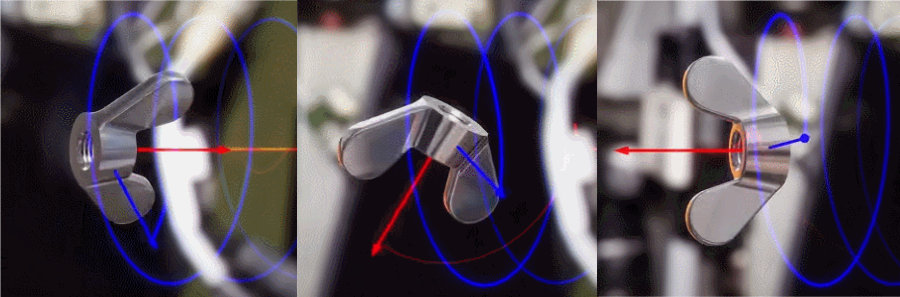
\includegraphics[width=0.9\textwidth]{dzhani.jpg}
\end{center}
   \caption{ジャンニベコフ効果の描写 \cite{28}。}
\label{fig:10}
\end{figure*}

世界の主要な砂漠と生物多様性ホットスポットの位置もこのパターンと一致している。砂漠は堆積物で大量に覆われることが予想される場所に存在し、一方で生物多様性ホットスポットは海洋の置換によってあまり影響を受けない地域に存在する \cite{28}。この一致は図 \ref{fig:9} に示されている。

予測されたECDO回転軸へのこうした一致は、アメリカ西部の砂岩層に保存されている堆積古流や、氷河または氷河によって持ち上げられ、異なる岩タイプの地層上に異質に置かれた岩塊(氷河漂着岩)に存在する。\cite{21} 英国では、これらの漂着岩はECDO回転と一致した流路をたどる。\cite{67,68} 

\section{ECDO反転の物理的因果関係}

地球の回転軸の急速な変化の背後にある原理は、回転する物体の物理学にある。この典型的な例がジャンニベコフ効果であり、ロシアの宇宙飛行士ウラジーミル・ジャンニベコフによって発見された \cite{37}。図 \ref{fig:10} に示されているように、慣性の3つの主要軸の1つで完璧に回っていない物体は、固定された回転軸を維持しない。もし第2の主軸に近い状態で回転している場合、突然の回転変化を経験するように見える。それが地球の急速な反転中に起こると考えるわけではないが、外部からの力がない限り、回転の物理学だけが地球の回転軸の急速な変化を説明できる。

\begin{figure}[t]
\begin{center}
   \includegraphics[width=1\linewidth]{llvp.jpg}
\end{center}
   \caption{南アフリカの下にあるLLVPの詳細な視覚化\cite{28}。}
\label{fig:12}
\label{fig:onecol}
\end{figure}

正確に言えば、地球は単純で均一なジャンニベコフ効果を経験するわけではほぼない。もしそうであれば、地球の回転軸が時間経過に伴って徐々に変化していることを検出できるはずである。むしろ、地球はその物理的構造における周期的な突然の乱れを経験し、「外部回転体」(地殻/マントル)と「内部回転体」(核)の切り離しにつながる。外部からの入力がない限り、角運動量の保存法則は地球が突然に回転軸を変えることができないことを示しており、地球への外部衝撃を除いて、内外の回転体の切り離しは突然で急激な反転を引き起こす可能性の少ない要因の一つである。
地球内部の混乱を引き起こす特定のプロセスは、地球の中心を構成する鉄の構造の状態変化と考えられています(図\ref{fig:11})。内核は六方最密充填の鉄(Fe)で構成されています\cite{141}。この六方最密充填のFeが液体金属状態に変わると、運動エネルギーを放出し、外核に流れ込みます。この相変化は、コアの磁気透過率を低下させ、地磁気場を弱め、熱を放出し、マントル内にLLVP(広大な低速剪断領域)構造\cite{38}(図\ref{fig:12})を作り出し、深海を介して地表を加熱します。これらの傾向は、最近数世紀にわたってよく記録されており、この論文で後述されます。

\begin{figure*}[t]
\begin{center}
\includegraphics[width=1\textwidth]{layers.jpg}
\end{center}
   \caption{ECDOの変化を引き起こす内なる地球のプロセスの描写\cite{129}。}
\label{fig:11}
\end{figure*}

\begin{figure*}[b]
\begin{center}
\includegraphics[width=0.9\textwidth]{saa.jpg}
\end{center}
   \caption{1590年から2025年までの地磁気場の弱体化を示す描写。gufm1とIGRF-14モデルを使用して計算\cite{125,126}。}
\label{fig:14}
\end{figure*}


地球内部の同じプロセスが逆の形で発生し、ECDO変化が発生した直後に地球の現在の回転状態に戻ると考えられています。

\section{差し迫った地球の反転の証拠}

私たちがもう一つの地球の反転の瀬戸際にいると信じる強い理由があります。地球規模の大変動は数千年間発生しておらず、これは歴史的な記録とデータに基づくと、これらのイベントが発生する頻度とほぼ一致しています。差し迫った反転を支持する最も強力なデータは、最近の地磁気データから来ており、地球の地磁気場が約二千年間弱まっていることを示しています。この弱体化は加速しており、ここ数十年で驚異的な速さに達しています。

図\ref{fig:14}で示されているのは、1590年と2025年の地球の地磁気場です\cite{125,126}。図に示されているように、地磁気場は大きく弱まっています。

地磁気場の弱体化のもう一つの指標は地磁気北極の位置です(図\ref{fig:13})。地磁気北極は歴史的にカナダの北極圏に位置していました。しかし、過去数世紀にわたりゆっくりと移動しており、数十年前に大きく加速しました。現在、それは年間55キロメートルの速度でロシアに急速に向かっています\cite{124}。


\begin{figure}[t]
\begin{center}
   \includegraphics[width=1\linewidth]{npw.jpg}
\end{center}
   \caption{1590年から2025年までの地磁気北極の位置、5年ごとの増分で描写\cite{142}。}
\label{fig:13}
\label{fig:onecol}
\end{figure}

\begin{figure}[t]
\begin{center}
   \includegraphics[width=1\linewidth]{ocean-highlight.jpg}
\end{center}
   \caption{1991年から2010年までの深層(深さ$>$2000 m)海洋の温暖化率、赤で囲んだ場所\cite{132}。}
\label{fig:15}
\label{fig:onecol}
\end{figure}

地球の磁場は内なるダイナモ、つまり地球の外核での回転により移動するマグマの流れの円柱によって生成されていると考えられています\cite{123}。弱体化する地磁気場は、地球内部深くでの混乱の兆候です。ECDO理論によれば、これらの混乱は熱を排出し、最終的にマントルとコアの分離を引き起こし、地球の反転をもたらします\cite{1}。
内核プロセスの存在を裏付けるかなりのデータがあります。温暖化する地球は、上昇する大陸および海洋の表面温度\cite{127,128}、地球の熱状流と同調して移動する大気中のCO2レベルの上昇\cite{129,130}、および世界的な海氷範囲の減少によって記録されています\cite{131}。データは、上昇するCO2レベルと温度が「人為的」気候変動の原因ではなく、むしろ外熱性のコアの下流影響であることを示唆しています\cite{129}。

最も重要なことに、深海(深さ $>$2000 メートル)での温暖化率の研究は、深海は温暖化しているだけでなく、最も強い温暖化率が深海層(4000 - 6000 m)で発見されることを示しています。この深海の温暖化は4000メートル未満に重心がある\cite{132,129}であり、大気によって上から海洋が加熱されているのであれば不可能です。このようなデータは、最近の気候および地磁気変化が地球の深部内部プロセスによって引き起こされているという強力な支持を提供します。図\ref{fig:15}は、1991年から2010年までの世界の深海温暖化率を示しています\cite{132}。

\section{差し迫る地球反転のモデリング}

\begin{figure}[b]
\begin{center}
   \includegraphics[width=1\linewidth]{saa-crop.jpeg}
\end{center}
   \caption{南大西洋異常に基づく転換点の計算は、2059年3月13日を指し示しています\cite{125,126}。}
\label{fig:16}
\label{fig:onecol}
\end{figure}

地球の次の反転のタイミングを予測するのは複雑な作業です。現時点でこれに最適なモデルは、地球の地磁気場、つまり南大西洋異常(SAA)です。これは南大西洋上の地域で、最も弱い地磁気場強度を持ち、32,000ナノテスラ未満の場強度の地域として定義されています\cite{135}。これは1590年の最も弱い場値でした。南大西洋異常の表面積は1590年に地球表面の1\%から2025年には21\%にまで増加しました\cite{136}。

地球が反転する可能性のある時期を推定するために、複雑なシステムが臨界転移に接近するモデルとして、SAA表面範囲データにべき法則転換点方程式を適合させました。私の計算では、2059年3月13日の転換点の日付が予測されました(図\ref{fig:16})。この予測は、移行に近づくにつれてますます正確になります\cite{136}。

他の指標としては、回転軸の移動、天候異常、地震および火山のデータも、次の地球反転がいつ起こるかをより良く予測するのに役立ちます。

\section{ECDO歴史年表}

過去のECDOイベントの正確な年表を確立するのは難しいですが、少なくとも2つのECDOイベントが完新世の間に存在したようです。エジプトの司祭からヘロドトスが語った記録によると、\textit{"最初の王からこのヘファイストスの司祭が最後に治めるまでの間に、三百四十一世代の人間があった... この間、彼らは太陽が昇る場所から四度移動し、そして今沈む場所に2回昇り、そして今昇る場所から2回沈んだ"} \cite{32}。プラトンは紀元前5世紀に生きていたが\cite{111}、アトランティスを一昼夜で水没させた洪水の後に9,000年前に、\textit{"その後多くの洪水があり、山に生き残った残党は文字の技術を知らず、多くの世代にわたって生存手段を獲得することだけに専念していた"} \cite{112}。これは、約9700 BCEのヤンガー・ドライアスの終わり以来、2度以上の反転があったことを示唆しています。この論文全体および私の研究で取り上げた物理的証拠\cite{2}は、プラトンの主張を十分に裏付けています。

最も最近のECDOフリップの候補日は紀元前2300年から1600年の期間です。多くの壊滅的な洪水の記録(Gun-Yu \cite{113,114,115}, Ogyges \cite{116,117}, ペルー \cite{118,119}, 出エジプト記 \cite{120})、文明の破壊と放棄(モヘンジョ・ダロ \cite{121}, ミノア文明 \cite{100,101})および物理的異常(ボンドイベント \cite{122}, 4.2キロ年イベント \cite{90})の日付がこの時期に当てられています。この時期以降に大きな壊滅的事件を示す十分な証拠の収束は見られません。

\section{結論}

オペレーションNANOOKは、WWII後に米国が北極圏とソ連北岸を地図化するための冷戦時代の偵察活動でした \cite{137}。調査中、磁極が以前の探検からの発見に基づいて設置されるべき場所よりも北に125〜200マイル移動していることが判明しました。これに従い、\textit{"政府の科学者たちの間で、磁極と地理極が一致したときに何が起こるのかという疑問が起こりました。これに答えるために、Paul A. Siple博士のプロジェクト管理の下、ランドコーポレーションは地球のモデルを使用して実験室研究を行う契約を結びました。これらのモデルは、電磁的に帯電した溶鉄の核を表わす内球と、地理的な極軸の周りを回転する地殻を表わす外球から成っていました。繰り返しの実験により、「磁極」が「地理極」に接近するにつれて、「磁極」は遠心力によって「地理極」に引き寄せられるようにその収束速度を加速させ、一致するように跳躍することが判明しました。しかし、実際には極が一致することはなく、「磁極」は「地理極」の周りを急速に「フリップ」し、遠心力で赤道に向かって回転し、その後、2つの軸が約89度の角度で分岐する位置に行き着くとのことでした。この極の「フリップ」が発生した後、軸は長い時間をかけて再び徐々に収束し始めます"} \cite{138,139}。

その後、\textit{"1948年初頭にペンタゴンでメジャー・ホワイトが出席した科学会議で、科学者たちは差し迫った極の反転現象を公に警告することの理由について議論しました。科学者たちは情報を公から隠すことに同意しませんでしたが、情報をどのように公表するかについても意見が一致しませんでした。ある科学者たちは、この現象の知識自体が社会の道徳的基盤を破壊する可能性があると感じていました。これらの恐れは1950年代初頭にフリップ現象についての情報が新聞欄と雑誌記事で公表されたが、驚くべきことに、地域的または疑い深い公衆からの反応はなく、彼らの恐れは根拠のないものであることが判明しました"} \cite{138,139}。

なぜ私たちはこれに注意を払わないのでしょうか?地球が以前に反転したという十分な理由があります。この論文は、論文の第2部とともに、その証拠が結集していることを示唆する多くの領域からの強力な証拠の要約を提供しています。世界中の洪水の物語、大陸を覆う塩と海の化石、古代の地下シェルター、動物の遺骸、そして壊滅的な地質学的風景などがあります。人類は数十万年前から存在するとされているにもかかわらず、現代の歴史は数千年前までしか遡れません。定期的に地球がひっくり返り、大陸が一掃され、私たちは石器時代に戻ってゼロから再出発することを余儀なくされ、古代史の記録がわずかな壊滅的物語に減少する可能性があるのでしょうか?もしそうであるならば、これを再び防ぐことは人類の最も重要な課題の一つであるかもしれません。

最後に、プラトンが著した「ティマイオス」において語られている、アテナイの政治家ソロンとエジプトの僧侶との対話をお伝えします。\cite{140} ソロンが古代史について彼らを話に引き込みたいと思い、最も古い伝説、すなわち最初の人間とされたフォロネウスとニオベについて話そうとし、大洪水の後にデウカリオンとピュラがどのように生き延びたか、その子孫の系譜を語り、それにかかった年数を数えて時間の期間を計算しようとしました。その時、非常に年老いた僧侶の一人が言いました。「オー ソロン ソロン、あなたたちギリシャ人はいつも子供だ。老いたギリシャ人というものは決して存在しない。」 これを聞いたソロンは尋ねました。「この言葉で何を意味するのか?」 すると僧侶は答えました。「あなたたち皆が若い魂を持っている。そこには古代の伝統から受け継がれたものではない、古びた科学の一つも持っていない。そして、これがその理由です。人類には多くの、様々な破壊がありました。最も大きなものは火と水によるもので、より小さいものは数え切れない他の手段によります。真実、あなたたちの国でも我々の国でも語られている物語、かつてパエトンが父ヘリオスの馬車を引き、その父の通り道に沿ってそれを運転できなかったために、地上のすべてを焼きつくし、雷電によって彼自身が滅びたという、その物語は伝説の様相をしていますが、その真実は天体の移動に関連した変動にあり、地上のものが猛火によって長い間隔をあけて繰り返し破壊されるという出来事にあります。その時には山岳地帯や高地や乾燥した地域に住む人々は、川や海の近くに住む人々よりも深刻な被害を受けますが、我々の場合、ナイルはこの時も我々を救い、この災いから守ってくれます。そしてまた一方で、神々が大洪水で地を浄化する時には、山岳地帯の全ての牧夫や羊飼いは生き残りますが、あなたたちの国の都市にいる人は全て流れに押し流され海に沈みます。我々の国では、逆に上方から水が我々の田畑に流れ込むことはなく、すべては自然に地下から湧き出る傾向があります。このため、ここで保存されるものが最も古いと言われているのです。そして、どこであっても、過度な暑さや寒さが存在しないところには、常に人の種族が少なかれ多かれ存在しています。そして、もしあなたの国やわたしたちの国や、または報告によって知っている他の場所で高貴または偉大または目立った出来事が起こった場合、旧来からそれら全ての出来事はここ、我々の神殿に記録され保存されています。あなたたちの人々や他の国の人々は、文明国家が必要とする文字や芸術を新たに装備しており、通常の年数が経った後、天からの洪水が新たにやって来る度に、それはあなたたちを字を書けない、文化的でない者だけを残して襲い、かくしてあなた達は古代にこの土地や自国で起こった全ての出来事を知らずに、常に若返るのです。確かに、数分前にあなたが語った系譜に関しては、ソロン、あなたたちの国の人々に関するそれは、子供の物語程度のものでした; なぜなら、まず一つには、あなたたちは一つの洪水しか思い出さないが、以前にも多くの洪水があったことがあり、次に、あなたたちは現人類の中で最も高貴で完璧な種族がかつて住んでいた場所に今住んでいることを知らないし、それからあなた自信が生まれ、そして残りのあなたたちの既存の都市が残っているのです。このことは、何世代も記録することのできる力なく生き残った人々が死亡してしまったために、気づきませんでした。本当にある時、ソロン、最大の水による破壊が起こる前、今のアテナイ国家が最も勇敢で戦争でも殊に組織化されており、また他のあらゆる面においても非常に優れていました。それは、天の下で聞いたことのあるどの国のどの国家も擁していなかった最も壮麗な芸術作品と高貴な国家体制を有していたと言われています」
もちろん、これらの同じ司祭たちはソロンにアトランティスの古代文明についても語りました:\textit{"私たちが話している口の中に横たわるすべてのものは、明らかに狭い入り口を持つ避難所です。しかし、向こうは本当の海であり、それを囲む土地は最も正確に、完全にして真実の意味で大陸と呼ばれるべきものです。さて、このアトランティスの島には、島全体および他の多くの島々と大陸の一部を支配していた偉大で驚異的な力を持つ王たちの同盟が存在しました。さらに、ストレートのこちら側の土地でも、彼らはリビアからエジプトまで、そしてヨーロッパからティレニアまで支配しました。それで、この軍勢がすべて集まって、ストレート内のあなたの国と私たちの国、および全地の奴隷にする試みを一度による攻撃で行いました。そしてその時、ソロンよ、あなたの国家の男らしさが全世界の目に勇気と力で顕著に現れました。それはすべての中で勇敢さとすべての戦闘技術において並外れて立ち、ギリシャ人の一部としてリーダーとして行動し、他のすべてに見捨てられたときには単独で立ち、最も致命的な危険に立ち向かった後、侵略者を打ち負かし、戦利品を築き、それによりまだ奴隷とされていない者たちを奴隷から救い、ヘラクレスの領域内に住む私たちを惜しみなく自由にしました。しかし、後の時代に、途方もない地震と洪水が起こり、厳しい一日と夜が彼らに降りかかり、あなたの戦士たち全体が地中に呑み込まれ、同様にアトランティスの島も海に呑み込まれ消失しました"}.

\section{謝辞}

最初のECDO論文の著者であるEthical Skeptic氏に感謝します。その洞察に満ちた画期的な論文を完成させ、世界と共有してくれました。彼の三部作の論文\cite{1}は、Exothermic Core-Mantle Decoupling Dzhanibekov Oscillation(ECDO)理論の基本的な著作であり、ここで簡単に取り上げた以上の情報が含まれています。

表1の大惨事データを処理してくれたAnkitに感謝します。

そしてもちろん、私たちが立っている巨人たちに感謝します。この研究を可能にしたすべての調査と研究を行い、人類に光をもたらすために働いた人々に感謝します。

\clearpage
\twocolumn

\section{追加画像}

\begin{figure}[H]
\begin{center}
   \includegraphics[width=1\linewidth]{wave.jpg}
\end{center}
   \caption{カフラー王のピラミッドにおける、引き込み部の放物線状の波侵食のクローズアップ\cite{27}。}
\label{fig:19}
\label{fig:onecol}
\end{figure}

\begin{figure}[H]
\begin{center}
   \includegraphics[width=1\linewidth]{star-stone.jpg}
\end{center}
   \caption{クフ王のピラミッド内のシャフトの一つに石に刻まれた星図\cite{28}。}
\label{fig:20}
\label{fig:onecol}
\end{figure}

\begin{figure*}[t]
\begin{center}
\includegraphics[width=1\textwidth]{deepsea.jpg}
\end{center}
   \caption{深海と深海底の加熱異常と通常の大気海洋加熱曲線の比較視覚化。全体的な加熱異常はNOAAから得られ\cite{147}、深海と深海底の加熱分布はDesbruyeresの研究から、データ処理と視覚化はEthical Skepticによるものです\cite{132,129}。}
\label{fig:21}
\end{figure*}

\begin{figure*}[t]
\begin{center}
\includegraphics[width=1\textwidth]{sealevel.jpeg}
\end{center}
   \caption{海面は63の観測所で75年間で20\%の変動増加を示し、流速の増加を示しています。海面変動の急増は海洋加熱パルスと同時に発生しており、これらは地球の海の深部からの加熱によって引き起こされている可能性が示唆されます\cite{2,129}。}
\label{fig:22}
\end{figure*}
\begin{figure*}[t]
\begin{center}
\includegraphics[width=1\textwidth]{co2.jpg}
\end{center}
   \caption{大気中のCO2濃度(ppm)は過去45年間で一貫して上昇しており、これは海洋温度の上昇が原因と考えられます。出典:NOAA \cite{148,129}.}
\label{fig:23}
\end{figure*}

\begin{figure*}[t]
\begin{center}
\includegraphics[width=1\textwidth]{ice.jpg}
\end{center}
   \caption{地球温暖化の影響で、過去45年間で全球の海氷範囲が縮小しています。出典:ADS \cite{149}.}
\label{fig:24}
\end{figure*}

\clearpage
\twocolumn

{\small
\bibliographystyle{ieee}
\bibliography{egbib}
}

\end{document}
